\chapter{Estudio de requisitos}

\section{Actores}

\begin{table}[H]
    \begin{tabular}{|llllll|}
	\hline
	\multicolumn{1}{|l|}{\textbf{Actor}}		& \multicolumn{4}{l|}{Desarrollador}	& AC-01	    \\ \hline
	\multicolumn{1}{|l|}{\textbf{Descripción}}     	& \multicolumn{5}{l|}{Persona que utiliza el port para hacer un proyecto con la placa}	    \\ \hline
	\multicolumn{1}{|l|}{\textbf{Características}}	& \multicolumn{5}{l|}{Programar}	\\ \hline
	\multicolumn{1}{|l|}{\textbf{Relaciones}}		& \multicolumn{5}{l|}{Diseña tareas que luego FreeRTOS ejecuta}	    \\ \hline
	\multicolumn{1}{|l|}{\textbf{Referencias}}     	& \multicolumn{5}{l|}{???}	\\ \hline
	\multicolumn{1}{|l|}{\textbf{Autor}}           	& \multicolumn{1}{l|}{Enrique Paubert}        & \multicolumn{1}{l|}{\textbf{Fecha}}        & \multicolumn{1}{l|}{10/08/2024}        & \multicolumn{1}{l|}{\textbf{Versión}}       & 1.0                   \\ \hline
	\multicolumn{6}{|l|}{\textbf{\underline{Atributos}}} \\ \hline % \cellcolor[HTML]{DAE8FC}
	\multicolumn{1}{|l|}{\textbf{Nombre}}		& \multicolumn{4}{l|}{\textbf{Descripción}} &  \textbf{Tipo}  \\ \hline
	\multicolumn{1}{|l|}{ ??? }				& \multicolumn{4}{l|}{ ??? }  &  ???      \\ \hline
    \end{tabular}
    \caption[Actor: Desarrollador]{Especificación del actor Desarrollador. Elaboración propia}
\end{table}

\begin{table}[H]
    \begin{tabular}{|llllll|}
	\hline
	\multicolumn{1}{|l|}{\textbf{Actor}}		& \multicolumn{4}{l|}{RTOS} & AC-02		\\ \hline
	\multicolumn{1}{|l|}{\textbf{Descripción}}     	& \multicolumn{5}{l|}{El sistema operativo}	\\ \hline
	\multicolumn{1}{|l|}{\textbf{Características}}	& \multicolumn{5}{l|}{Gestiona las tareas}	\\ \hline
	\multicolumn{1}{|l|}{\textbf{Relaciones}}		& \multicolumn{5}{l|}{Hace que la placa ejecute las tareas programadas por el desarrollador}	\\ \hline
	\multicolumn{1}{|l|}{\textbf{Referencias}}     	& \multicolumn{5}{l|}{???}	\\ \hline
	\multicolumn{1}{|l|}{\textbf{Autor}}           	& \multicolumn{1}{l|}{Enrique Paubert}        & \multicolumn{1}{l|}{\textbf{Fecha}}        & \multicolumn{1}{l|}{10/08/2024}        & \multicolumn{1}{l|}{\textbf{Versión}}       & 1.0                   \\ \hline
	\multicolumn{6}{|l|}{\textbf{\underline{Atributos}}} \\ \hline % \cellcolor[HTML]{DAE8FC}
	\multicolumn{1}{|l|}{\textbf{Nombre}}		& \multicolumn{4}{l|}{\textbf{Descripción}} &  \textbf{Tipo}  \\ \hline
	\multicolumn{1}{|l|}{ Alias }				& \multicolumn{4}{l|}{ FreeRTOS }  &  string      \\ \hline
    \end{tabular}
    \caption[Actor: RTOS]{Especificación del actor RTOS. Elaboración propia}
\end{table}

\begin{table}[H]
    \begin{tabular}{|llllll|}
	\hline
	\multicolumn{1}{|l|}{\textbf{Actor}}		& \multicolumn{4}{l|}{Placa} & AC-03		\\ \hline
	\multicolumn{1}{|l|}{\textbf{Descripción}}     	& \multicolumn{5}{l|}{Placa sobre la que se desarrolla el proyecto}	\\ \hline
	\multicolumn{1}{|l|}{\textbf{Características}}	& \multicolumn{5}{l|}{Realiza las tareas}	\\ \hline
	\multicolumn{1}{|l|}{\textbf{Relaciones}}		& \multicolumn{5}{l|}{Se ejecutan sobre ella las tareas}	\\ \hline
	\multicolumn{1}{|l|}{\textbf{Referencias}}     	& \multicolumn{5}{l|}{???}	\\ \hline
	\multicolumn{1}{|l|}{\textbf{Autor}}           	& \multicolumn{1}{l|}{Enrique Paubert}        & \multicolumn{1}{l|}{\textbf{Fecha}}        & \multicolumn{1}{l|}{10/08/2024}        & \multicolumn{1}{l|}{\textbf{Versión}}       & 1.0                   \\ \hline
	\multicolumn{6}{|l|}{\textbf{\underline{Atributos}}} \\ \hline % \cellcolor[HTML]{DAE8FC}
	\multicolumn{1}{|l|}{\textbf{Nombre}}		& \multicolumn{4}{l|}{\textbf{Descripción}} &  \textbf{Tipo}  \\ \hline
	\multicolumn{1}{|l|}{ ??? }				& \multicolumn{4}{l|}{ ??? }  & ???	\\ \hline
    \end{tabular}
    \caption[Actor: Placa]{Especificación del actor Placa. Elaboración propia}
\end{table}

\section{Casos de Uso}

\begin{table}[H]
    \begin{tabular}{|l|l|l|l|l|l|}
	\hline
	\textbf{Caso de Uso} & \multicolumn{3}{l|}{Crear una tarea} & \multicolumn{2}{l|}{CU-01} \\ \hline
	\textbf{Actores} & \multicolumn{5}{l|}{Desarrollador, RTOS} \\ \hline
	\textbf{Tipo} & \multicolumn{5}{l|}{Primario, Esencial} \\ \hline
	\textbf{Referencias} & RF1 & \multicolumn{4}{l|}{???} \\ \hline
	\textbf{Precondición} & \multicolumn{5}{l|}{???} \\ \hline
	\textbf{Postcondición} & \multicolumn{5}{l|}{Habrá una nueva tarea} \\ \hline
	\textbf{Autor} & Enrique Paubert & \textbf{Fecha} & 10/08/2024 & \textbf{Versión} & v.1 \\ \hline
	\multicolumn{6}{|l|}{\textbf{\underline{Propósito}}} \\ \hline %\cellcolor[HTML]{ECF4FF}
	\multicolumn{6}{|l|}{El desarrollador diseña una tarea, se añade al planificador de FreeRTOS} \\ \hline
	\multicolumn{6}{|l|}{\textbf{\underline{Resumen}}} \\ \hline % \cellcolor[HTML]{ECF4FF}
	\multicolumn{6}{|l|}{\begin{tabular}[c]{@{}l@{}}1. El desarollador crea una tarea.\\  2. ???. \\ 3. profit.\end{tabular}} \\ \hline
    \end{tabular}%
\end{table}

\begin{table}[H]
    \begin{tabular}{|l|l|l|l|l|l|}
	\hline
	\textbf{Caso de Uso} & \multicolumn{3}{l|}{Configurara una tarea} & \multicolumn{2}{l|}{CU-02} \\ \hline
	\textbf{Actores} & \multicolumn{5}{l|}{Desarrollador, RTOS} \\ \hline
	\textbf{Tipo} & \multicolumn{5}{l|}{Primario, Esencial} \\ \hline
	\textbf{Referencias} & RF1 & \multicolumn{4}{l|}{???} \\ \hline
	\textbf{Precondición} & \multicolumn{5}{l|}{Existe una tarea} \\ \hline
	\textbf{Postcondición} & \multicolumn{5}{l|}{La configuración de dicha tarea cambia} \\ \hline
	\textbf{Autor} & Enrique Paubert & \textbf{Fecha} & 10/08/2024 & \textbf{Versión} & v.1 \\ \hline
	\multicolumn{6}{|l|}{\textbf{\underline{Propósito}}} \\ \hline %\cellcolor[HTML]{ECF4FF}
	\multicolumn{6}{|l|}{El desarrollador configura una tarea, el RTOS recibe esa configuración} \\ \hline
	\multicolumn{6}{|l|}{\textbf{\underline{Resumen}}} \\ \hline % \cellcolor[HTML]{ECF4FF}
	\multicolumn{6}{|l|}{\begin{tabular}[c]{@{}l@{}}1. El desarollador configura una tarea.\\  2. ???. \\ 3. profit.\end{tabular}} \\ \hline
    \end{tabular}%
\end{table}

\begin{table}[H]
    \begin{tabular}{|l|l|l|l|l|l|}
	\hline
	\textbf{Caso de Uso} & \multicolumn{3}{l|}{Configurar el sistema} & \multicolumn{2}{l|}{CU-03} \\ \hline
	\textbf{Actores} & \multicolumn{5}{l|}{Desarrollador, RTOS} \\ \hline
	\textbf{Tipo} & \multicolumn{5}{l|}{Primario, Esencial} \\ \hline
	\textbf{Referencias} & RF1 & \multicolumn{4}{l|}{???} \\ \hline
	\textbf{Precondición} & \multicolumn{5}{l|}{El sistema tiene una configuración concreta} \\ \hline
	\textbf{Postcondición} & \multicolumn{5}{l|}{La configuración del sistema ha cambiado} \\ \hline
	\textbf{Autor} & Enrique Paubert & \textbf{Fecha} & 10/08/2024 & \textbf{Versión} & v.1 \\ \hline
	\multicolumn{6}{|l|}{\textbf{\underline{Propósito}}} \\ \hline %\cellcolor[HTML]{ECF4FF}
	\multicolumn{6}{|l|}{Que el desarrollador pueda configurar el sistema según sus necesidades} \\ \hline
	\multicolumn{6}{|l|}{\textbf{\underline{Resumen}}} \\ \hline % \cellcolor[HTML]{ECF4FF}
	\multicolumn{6}{|l|}{\begin{tabular}[c]{@{}l@{}}1. El desarollador configura el sistema.\\  2. ???. \\ 3. profit.\end{tabular}} \\ \hline
    \end{tabular}%
\end{table}

\begin{table}[H]
    \begin{tabular}{|l|l|l|l|l|l|}
	\hline
	\textbf{Caso de Uso} & \multicolumn{3}{l|}{ Comunicación entre tareas } & \multicolumn{2}{l|}{CU-04} \\ \hline
	\textbf{Actores} & \multicolumn{5}{l|}{RTOS} \\ \hline
	\textbf{Tipo} & \multicolumn{5}{l|}{Primario, Esencial} \\ \hline
	\textbf{Referencias} & RF1 & \multicolumn{4}{l|}{???} \\ \hline
	\textbf{Precondición} & \multicolumn{5}{l|}{Existen 2 o más tareas} \\ \hline
	\textbf{Postcondición} & \multicolumn{5}{l|}{Una tarea ha modificado la ejecución de otra} \\ \hline
	\textbf{Autor} & Enrique Paubert & \textbf{Fecha} & 10/08/2024 & \textbf{Versión} & v.1 \\ \hline
	\multicolumn{6}{|l|}{\textbf{\underline{Propósito}}} \\ \hline %\cellcolor[HTML]{ECF4FF}
	\multicolumn{6}{|l|}{La utilización de una tarea para modificar otras tareas en tiempo real} \\ \hline
	\multicolumn{6}{|l|}{\textbf{\underline{Resumen}}} \\ \hline % \cellcolor[HTML]{ECF4FF}
	\multicolumn{6}{|l|}{\begin{tabular}[c]{@{}l@{}}1. Una tarea se está ejecutando\\  2. ???. \\ 3. profit.\end{tabular}} \\ \hline
    \end{tabular}%
\end{table}

\begin{table}[H]
    \begin{tabular}{|l|l|l|l|l|l|}
	\hline
	\textbf{Caso de Uso} & \multicolumn{3}{l|}{ Medición del tiempo } & \multicolumn{2}{l|}{CU-05} \\ \hline
	\textbf{Actores} & \multicolumn{5}{l|}{RTOS} \\ \hline
	\textbf{Tipo} & \multicolumn{5}{l|}{Primario, Esencial} \\ \hline
	\textbf{Referencias} & RF1 & \multicolumn{4}{l|}{???} \\ \hline
	\textbf{Precondición} & \multicolumn{5}{l|}{ ??? } \\ \hline
	\textbf{Postcondición} & \multicolumn{5}{l|}{ ??? } \\ \hline
	\textbf{Autor} & Enrique Paubert & \textbf{Fecha} & 10/08/2024 & \textbf{Versión} & v.1 \\ \hline
	\multicolumn{6}{|l|}{\textbf{\underline{Propósito}}} \\ \hline %\cellcolor[HTML]{ECF4FF}
	\multicolumn{6}{|l|}{El RTOS debe de tener un mecanismo para medir el paso del tiempo} \\ \hline
	\multicolumn{6}{|l|}{\textbf{\underline{Resumen}}} \\ \hline % \cellcolor[HTML]{ECF4FF}
	\multicolumn{6}{|l|}{\begin{tabular}[c]{@{}l@{}}1. Ticks. \\  2. ???. \\ 3. profit.\end{tabular}} \\ \hline
    \end{tabular}%
\end{table}

\section{Diagramas de casos de uso}

\begin{figure}[h]
\centering
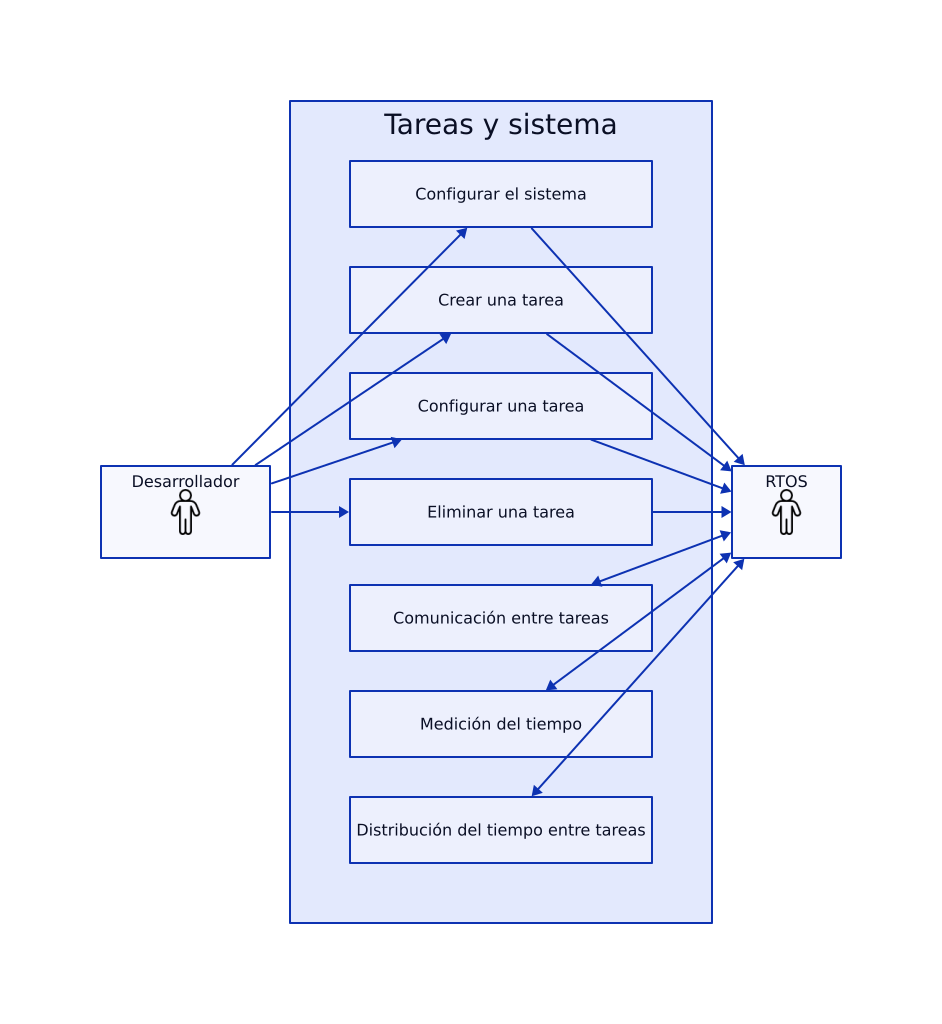
\includegraphics[width=\textwidth]{img/UML1.png}
\caption{Diagrama UML de las tareas}
\label{fig:UML1}
\end{figure}

\section{Requisitos}
\subsection{Requisitos funcionales}

\subsubsection{Soporte de Periféricos}
Integrando el BSP en el port, daremos soporte a los periféricos.

\subsubsection{Soporte de tareas concurrentes}
El RTOS soportará la ejecución de tareas concurrentes.

\subsubsection{Gestión de interrupciones}
El RTOS soportará la gestión de interrupciones.


\subsection{Requisitos no funcionales}
\subsubsection{Eficiencia y Rendimiento}
\subsubsection{Estabilidad y Robustez}

